\documentclass[a4paper, UTF-8]{article}
\usepackage{algorithm}
\usepackage{algpseudocode}
\usepackage{amsmath}
\usepackage{amsfonts}
\usepackage{amsthm}
\usepackage{tikz}
\usetikzlibrary{automata, positioning, arrows, trees, arrows.meta}
\usepackage[utf8]{inputenc}
\usepackage[T1]{fontenc}
\usepackage{hyperref}
\usepackage{url}
\usepackage{booktabs}
\usepackage{microtype}
\usepackage{xcolor}
\usepackage{amssymb}

\theoremstyle{plain}
\newtheorem{theorem}{\indent Theorem}[section]
\newtheorem{lemma}[theorem]{\indent Lemma}
\newtheorem{assumption}{\indent Assumption}[section]
\newtheorem{note}[theorem]{\indent Notation}
\newtheorem{proposition}[theorem]{\indent Proposition}
\newtheorem{corollary}[theorem]{\indent Corollary}
\newtheorem{definition}{\indent Definition}[section]
\newtheorem{example}{\indent Example}[section]
\newtheorem{remark}{\indent Remark}[section]
\newenvironment{solution}{\begin{proof}[\indent\bf Solution]}{\end{proof}}
\renewcommand{\proofname}{\indent\bf Proof}

\begin{document}

\title{\bf{Lab 12 Answers}}
\author{Yanqiao Chen\\ 
  Department of Computer Science and Engineering\\
  Southern University of Science and Technology\\
  \texttt{12412115@mail.sustech.edu.cn}
  }
\maketitle

\section{Question 1} 

\[
  \phi=(x\vee \bar y\vee \bar z)\wedge(\bar x\vee y\vee z)\wedge
  (\bar x\vee \bar y\vee \bar z).
\]

\begin{solution}
For the reduction from $3SAT$ to $3CLIQUE$, create one vertex for each
literal occurrence in each clause. Join two vertices by an edge if and only if
they come from different clauses and their literals are not contradictory.
Thus the target clique size is
\[
  k=3.
\]

Let
\[
  C_1=(x\vee \bar y\vee \bar z),\qquad
  C_2=(\bar x\vee y\vee z),\qquad
  C_3=(\bar x\vee \bar y\vee \bar z).
\]
The corresponding graph is:

\begin{center}
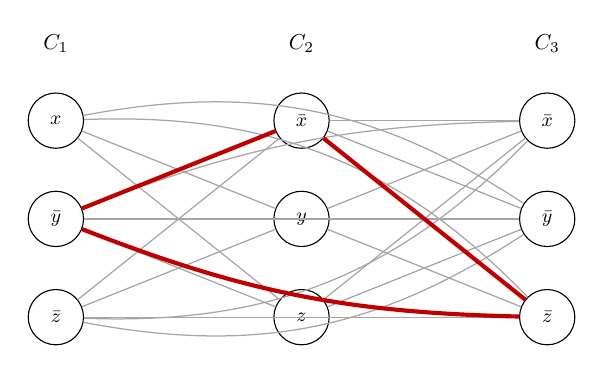
\begin{tikzpicture}[
  scale=0.78,
  transform shape,
  vertex/.style={circle, draw, minimum size=9mm, inner sep=0pt, font=\small},
  edge/.style={draw=black!35, line width=0.45pt},
  chosen/.style={draw=red!75!black, line width=1.5pt}
]
  \node[font=\bfseries] at (0,2.85) {$C_1$};
  \node[font=\bfseries] at (4,2.85) {$C_2$};
  \node[font=\bfseries] at (8,2.85) {$C_3$};

  \node[vertex] (c1x) at (0,1.6) {$x$};
  \node[vertex] (c1ny) at (0,0) {$\bar y$};
  \node[vertex] (c1nz) at (0,-1.6) {$\bar z$};

  \node[vertex] (c2nx) at (4,1.6) {$\bar x$};
  \node[vertex] (c2y) at (4,0) {$y$};
  \node[vertex] (c2z) at (4,-1.6) {$z$};

  \node[vertex] (c3nx) at (8,1.6) {$\bar x$};
  \node[vertex] (c3ny) at (8,0) {$\bar y$};
  \node[vertex] (c3nz) at (8,-1.6) {$\bar z$};

  % Compatible edges between C1 and C2.
  \draw[edge] (c1x) -- (c2y);
  \draw[edge] (c1x) -- (c2z);
  \draw[edge] (c1ny) -- (c2nx);
  \draw[edge] (c1ny) -- (c2z);
  \draw[edge] (c1nz) -- (c2nx);
  \draw[edge] (c1nz) -- (c2y);

  % Compatible edges between C2 and C3.
  \draw[edge] (c2nx) -- (c3nx);
  \draw[edge] (c2nx) -- (c3ny);
  \draw[edge] (c2nx) -- (c3nz);
  \draw[edge] (c2y) -- (c3nx);
  \draw[edge] (c2y) -- (c3nz);
  \draw[edge] (c2z) -- (c3nx);
  \draw[edge] (c2z) -- (c3ny);

  % Compatible edges between C1 and C3.
  \draw[edge] (c1x) to[bend left=22] (c3ny);
  \draw[edge] (c1x) to[bend left=24] (c3nz);
  \draw[edge] (c1ny) to[bend left=10] (c3nx);
  \draw[edge] (c1ny) -- (c3ny);
  \draw[edge] (c1ny) to[bend right=10] (c3nz);
  \draw[edge] (c1nz) to[bend right=24] (c3nx);
  \draw[edge] (c1nz) to[bend right=22] (c3ny);
  \draw[edge] (c1nz) -- (c3nz);

  % One valid 3-clique, corresponding to a satisfying choice of literals.
  \draw[chosen] (c1ny) -- (c2nx);
  \draw[chosen] (c2nx) -- (c3nz);
  \draw[chosen] (c1ny) to[bend right=10] (c3nz);
\end{tikzpicture}
\end{center}

The red triangle is one $3$-clique:
\[
  \{\bar y\in C_1,\ \bar x\in C_2,\ \bar z\in C_3\}.
\]
Since these three literals are mutually consistent, they correspond to a
satisfying choice for the three clauses.
\end{solution}

\section{Question 2} 

\begin{solution}
Let the input $2SAT$ formula be
\[
  \phi=C_1\wedge C_2\wedge \cdots \wedge C_m,
\]
where each clause has two literals:
\[
  C_i=(\ell_{i,1}\vee \ell_{i,2}).
\]
We construct a graph $G$ as follows.

\begin{itemize}
  \item For each literal occurrence $\ell_{i,j}$ in clause $C_i$, create one
  vertex $v_{i,j}$.
  \item Add an edge between $v_{i,j}$ and $v_{p,q}$ if $i\neq p$ and the two
  corresponding literals are not contradictory. That is, we do not connect
  $x$ with $\bar x$.
  \item Set the clique size to be
  \[
    k=m.
  \]
\end{itemize}

We now prove correctness.

If $\phi$ is satisfiable, then every clause has at least one true literal.
Choose one true literal from each clause. These $m$ chosen literals are from
different clauses, and no two of them can be contradictory, since they are all
true under the same assignment. Therefore, the corresponding $m$ vertices are
pairwise adjacent, so they form a clique of size $m$.

Conversely, suppose $G$ has a clique of size $m$. Since vertices from the same
clause are not connected, the clique can contain at most one vertex from each
clause. There are $m$ clauses and the clique has size $m$, so it contains
exactly one vertex from each clause. Also, since every pair of vertices in the
clique is connected, the corresponding literals are mutually consistent.
Thus we can assign variables so that all these chosen literals are true. Then
each clause has at least one true literal, so $\phi$ is satisfiable.

The construction creates $2m$ vertices and at most $O(m^2)$ edges, so it runs in
polynomial time. Hence
\[
  2SAT\le_p CLIQUE.
\]

After obtaining this correct reduction, we can conclude that every $2SAT$
instance can be transformed into an equivalent $CLIQUE$ instance in polynomial
time. However, since $2SAT\in P$, this reduction alone does not prove that
$CLIQUE$ is NP-hard. To prove $CLIQUE$ is NP-hard, we need a reduction from an
NP-complete problem such as $3SAT$.
\end{solution}

\section{Question 3}

\[
  \phi=(x\vee y)\wedge(\bar x\vee y)\wedge
  (\bar x\vee \bar y)\wedge(\bar x\vee \bar y).
\]

\begin{solution}
Let
\[
  C_1=(x\vee y),\quad
  C_2=(\bar x\vee y),\quad
  C_3=(\bar x\vee \bar y),\quad
  C_4=(\bar x\vee \bar y).
\]
For the reduction to $CLIQUE$, create one vertex for each literal occurrence
and connect two vertices if they are from different clauses and are not
contradictory. Since there are four clauses, the target clique size is
\[
  k=4.
\]

\begin{center}
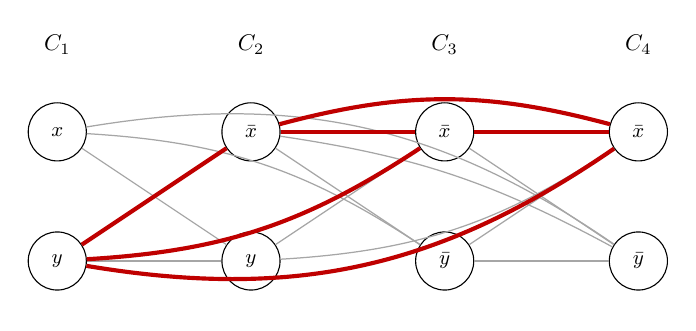
\begin{tikzpicture}[
  scale=0.82,
  transform shape,
  vertex/.style={circle, draw, minimum size=9mm, inner sep=0pt, font=\small},
  edge/.style={draw=black!35, line width=0.45pt},
  chosen/.style={draw=red!75!black, line width=1.5pt}
]
  \node[font=\bfseries] at (0,2.35) {$C_1$};
  \node[font=\bfseries] at (3,2.35) {$C_2$};
  \node[font=\bfseries] at (6,2.35) {$C_3$};
  \node[font=\bfseries] at (9,2.35) {$C_4$};

  \node[vertex] (c1x) at (0,1) {$x$};
  \node[vertex] (c1y) at (0,-1) {$y$};

  \node[vertex] (c2nx) at (3,1) {$\bar x$};
  \node[vertex] (c2y) at (3,-1) {$y$};

  \node[vertex] (c3nx) at (6,1) {$\bar x$};
  \node[vertex] (c3ny) at (6,-1) {$\bar y$};

  \node[vertex] (c4nx) at (9,1) {$\bar x$};
  \node[vertex] (c4ny) at (9,-1) {$\bar y$};

  % Compatible edges between C1 and C2.
  \draw[edge] (c1x) -- (c2y);
  \draw[edge] (c1y) -- (c2nx);
  \draw[edge] (c1y) -- (c2y);

  % Compatible edges between C1 and C3.
  \draw[edge] (c1x) to[bend left=15] (c3ny);
  \draw[edge] (c1y) to[bend right=15] (c3nx);

  % Compatible edges between C1 and C4.
  \draw[edge] (c1x) to[bend left=22] (c4ny);
  \draw[edge] (c1y) to[bend right=22] (c4nx);

  % Compatible edges between C2 and C3.
  \draw[edge] (c2nx) -- (c3nx);
  \draw[edge] (c2nx) -- (c3ny);
  \draw[edge] (c2y) -- (c3nx);

  % Compatible edges between C2 and C4.
  \draw[edge] (c2nx) to[bend left=15] (c4nx);
  \draw[edge] (c2nx) to[bend left=10] (c4ny);
  \draw[edge] (c2y) to[bend right=15] (c4nx);

  % Compatible edges between C3 and C4.
  \draw[edge] (c3nx) -- (c4nx);
  \draw[edge] (c3nx) -- (c4ny);
  \draw[edge] (c3ny) -- (c4nx);
  \draw[edge] (c3ny) -- (c4ny);

  % One 4-clique: y, not x, not x, not x.
  \draw[chosen] (c1y) -- (c2nx);
  \draw[chosen] (c1y) to[bend right=15] (c3nx);
  \draw[chosen] (c1y) to[bend right=22] (c4nx);
  \draw[chosen] (c2nx) -- (c3nx);
  \draw[chosen] (c2nx) to[bend left=15] (c4nx);
  \draw[chosen] (c3nx) -- (c4nx);
\end{tikzpicture}
\end{center}

The red vertices
\[
  \{y\in C_1,\ \bar x\in C_2,\ \bar x\in C_3,\ \bar x\in C_4\}
\]
form a $4$-clique. Therefore, the obtained graph contains a $4CLIQUE$.
This corresponds to the satisfying assignment, for example,
\[
  x=\text{false},\qquad y=\text{true}.
\]

The graph also contains a $3CLIQUE$, because any three vertices from the above
$4$-clique form a $3$-clique. For example,
\[
  \{y\in C_1,\ \bar x\in C_2,\ \bar x\in C_3\}
\]
is a $3$-clique.
\end{solution}

\section{Question 4}

\begin{solution}
First, we show that $\text{Double}-SAT$ is in NP. A certificate consists of two
different assignments $a_1$ and $a_2$. We can check in polynomial time that
$a_1\neq a_2$ and that both assignments satisfy $\phi$.

Then we reduce $3SAT$ to $\text{Double}-SAT$. Given a $3SAT$ formula $\phi$,
construct
\[
  \phi'=\phi\wedge (w\vee \bar w),
\]
where $w$ is a new variable that does not appear in $\phi$. This construction
is clearly polynomial time.

If $\phi$ is satisfiable, let $a$ be a satisfying assignment for $\phi$. Then
extending $a$ with $w=\text{true}$ satisfies $\phi'$, and extending $a$ with
$w=\text{false}$ also satisfies $\phi'$. Hence $\phi'$ has at least two
satisfying assignments.

Conversely, if $\phi'$ has at least two satisfying assignments, then $\phi'$ is
satisfiable. Since $(w\vee \bar w)$ is always true, the restriction of any
satisfying assignment of $\phi'$ to the variables of $\phi$ satisfies $\phi$.
Thus $\phi$ is satisfiable.

Therefore,
\[
  \phi\in 3SAT\iff \phi'\in \text{Double}-SAT.
\]
So $\text{Double}-SAT$ is NP-hard. Since it is also in NP, it is NP-complete.

\end{solution}

\section{Question 5}

\[
  \phi=(x\vee \bar y\vee z)\wedge(\bar x\vee y\vee z)\wedge
  (\bar x\vee \bar y\vee z).
\]

\begin{solution}
Let
\[
  C_1=(x\vee \bar y\vee z),\quad
  C_2=(\bar x\vee y\vee z),\quad
  C_3=(\bar x\vee \bar y\vee z).
\]
We construct a directed $HAMPATH$ instance using Sipser-style diamond variable
gadgets. Traversing a variable gadget from left to right represents assigning
the variable true, and traversing it from right to left represents assigning it
false. Clause vertices are connected to the corresponding literal positions in
the variable gadgets.

For example, the assignment
\[
  x=\text{false},\qquad y=\text{false},\qquad z=\text{true}
\]
satisfies all three clauses. The red path below is the corresponding
Hamiltonian path.

\begin{center}
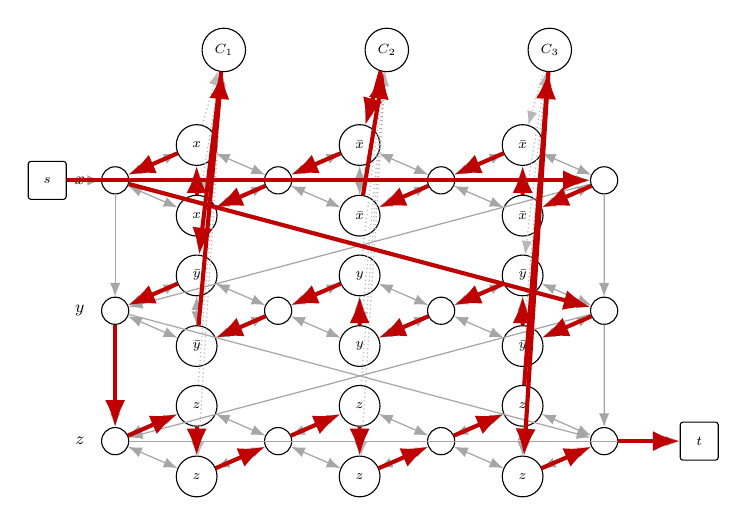
\begin{tikzpicture}[
  scale=0.69,
  transform shape,
  vertex/.style={circle, draw, minimum size=7.5mm, inner sep=0pt,
    font=\scriptsize, fill=white},
  joint/.style={circle, draw, minimum size=5mm, inner sep=0pt,
    font=\scriptsize, fill=white},
  endpoint/.style={rectangle, draw, rounded corners=1pt, minimum size=7mm,
    inner sep=1pt, font=\scriptsize, fill=white},
  clause/.style={circle, draw, minimum size=8mm, inner sep=0pt,
    font=\scriptsize, fill=white},
  edge/.style={draw=black!35, line width=0.45pt, <->, >=Latex},
  dir/.style={draw=black!35, line width=0.45pt, ->, >=Latex},
  wire/.style={draw=black!28, densely dotted, line width=0.45pt, ->, >=Latex},
  hpath/.style={draw=red!75!black, line width=1.5pt, ->, >=Latex}
]
  % Clause vertices.
  \node[clause] (c1) at (2.0,5.7) {$C_1$};
  \node[clause] (c2) at (5.0,5.7) {$C_2$};
  \node[clause] (c3) at (8.0,5.7) {$C_3$};

  % Start and terminal vertices.
  \node[endpoint] (s) at (-1.25,3.3) {$s$};
  \node[endpoint] (t) at (10.75,-1.5) {$t$};

  % x diamond gadget.
  \node[joint] (xL) at (0,3.3) {};
  \node[joint] (xM1) at (3,3.3) {};
  \node[joint] (xM2) at (6,3.3) {};
  \node[joint] (xR) at (9,3.3) {};
  \node[vertex] (xT1) at (1.5,3.95) {$x$};
  \node[vertex] (xB1) at (1.5,2.65) {$x$};
  \node[vertex] (xT2) at (4.5,3.95) {$\bar x$};
  \node[vertex] (xB2) at (4.5,2.65) {$\bar x$};
  \node[vertex] (xT3) at (7.5,3.95) {$\bar x$};
  \node[vertex] (xB3) at (7.5,2.65) {$\bar x$};
  \node[font=\small] at (-0.65,3.3) {$x$};

  % y diamond gadget.
  \node[joint] (yL) at (0,0.9) {};
  \node[joint] (yM1) at (3,0.9) {};
  \node[joint] (yM2) at (6,0.9) {};
  \node[joint] (yR) at (9,0.9) {};
  \node[vertex] (yT1) at (1.5,1.55) {$\bar y$};
  \node[vertex] (yB1) at (1.5,0.25) {$\bar y$};
  \node[vertex] (yT2) at (4.5,1.55) {$y$};
  \node[vertex] (yB2) at (4.5,0.25) {$y$};
  \node[vertex] (yT3) at (7.5,1.55) {$\bar y$};
  \node[vertex] (yB3) at (7.5,0.25) {$\bar y$};
  \node[font=\small] at (-0.65,0.9) {$y$};

  % z diamond gadget.
  \node[joint] (zL) at (0,-1.5) {};
  \node[joint] (zM1) at (3,-1.5) {};
  \node[joint] (zM2) at (6,-1.5) {};
  \node[joint] (zR) at (9,-1.5) {};
  \node[vertex] (zT1) at (1.5,-0.85) {$z$};
  \node[vertex] (zB1) at (1.5,-2.15) {$z$};
  \node[vertex] (zT2) at (4.5,-0.85) {$z$};
  \node[vertex] (zB2) at (4.5,-2.15) {$z$};
  \node[vertex] (zT3) at (7.5,-0.85) {$z$};
  \node[vertex] (zB3) at (7.5,-2.15) {$z$};
  \node[font=\small] at (-0.65,-1.5) {$z$};

  % Diamond edges for each variable gadget. A double arrow denotes two
  % opposite directed edges.
  \draw[edge] (xL)--(xT1); \draw[edge] (xT1)--(xM1);
  \draw[edge] (xM1)--(xB1); \draw[edge] (xB1)--(xL);
  \draw[edge] (xT1)--(xB1);
  \draw[edge] (xM1)--(xT2); \draw[edge] (xT2)--(xM2);
  \draw[edge] (xM2)--(xB2); \draw[edge] (xB2)--(xM1);
  \draw[edge] (xT2)--(xB2);
  \draw[edge] (xM2)--(xT3); \draw[edge] (xT3)--(xR);
  \draw[edge] (xR)--(xB3); \draw[edge] (xB3)--(xM2);
  \draw[edge] (xT3)--(xB3);

  \draw[edge] (yL)--(yT1); \draw[edge] (yT1)--(yM1);
  \draw[edge] (yM1)--(yB1); \draw[edge] (yB1)--(yL);
  \draw[edge] (yT1)--(yB1);
  \draw[edge] (yM1)--(yT2); \draw[edge] (yT2)--(yM2);
  \draw[edge] (yM2)--(yB2); \draw[edge] (yB2)--(yM1);
  \draw[edge] (yT2)--(yB2);
  \draw[edge] (yM2)--(yT3); \draw[edge] (yT3)--(yR);
  \draw[edge] (yR)--(yB3); \draw[edge] (yB3)--(yM2);
  \draw[edge] (yT3)--(yB3);

  \draw[edge] (zL)--(zT1); \draw[edge] (zT1)--(zM1);
  \draw[edge] (zM1)--(zB1); \draw[edge] (zB1)--(zL);
  \draw[edge] (zT1)--(zB1);
  \draw[edge] (zM1)--(zT2); \draw[edge] (zT2)--(zM2);
  \draw[edge] (zM2)--(zB2); \draw[edge] (zB2)--(zM1);
  \draw[edge] (zT2)--(zB2);
  \draw[edge] (zM2)--(zT3); \draw[edge] (zT3)--(zR);
  \draw[edge] (zR)--(zB3); \draw[edge] (zB3)--(zM2);
  \draw[edge] (zT3)--(zB3);

  % Choice and transition edges between gadgets.
  \draw[dir] (s)--(xL);
  \draw[dir] (s)--(xR);
  \draw[dir] (xL)--(yL);
  \draw[dir] (xL)--(yR);
  \draw[dir] (xR)--(yL);
  \draw[dir] (xR)--(yR);
  \draw[dir] (yL)--(zL);
  \draw[dir] (yL)--(zR);
  \draw[dir] (yR)--(zL);
  \draw[dir] (yR)--(zR);
  \draw[dir] (zL)--(t);
  \draw[dir] (zR)--(t);

  % Literal wires from clauses to matching literal positions.
  \draw[wire] (xT1)--(c1); \draw[wire] (c1)--(xB1);
  \draw[wire] (yB1)--(c1); \draw[wire] (c1)--(yT1);
  \draw[wire] (zT1)--(c1); \draw[wire] (c1)--(zB1);

  \draw[wire] (xB2)--(c2); \draw[wire] (c2)--(xT2);
  \draw[wire] (yT2)--(c2); \draw[wire] (c2)--(yB2);
  \draw[wire] (zT2)--(c2); \draw[wire] (c2)--(zB2);

  \draw[wire] (xB3)--(c3); \draw[wire] (c3)--(xT3);
  \draw[wire] (yB3)--(c3); \draw[wire] (c3)--(yT3);
  \draw[wire] (zT3)--(c3); \draw[wire] (c3)--(zB3);

  % Highlighted Hamiltonian path for x=false, y=false, z=true.
  \draw[hpath] (s)--(xR); \draw[hpath] (xR)--(xB3);
  \draw[hpath] (xB3)--(xT3); \draw[hpath] (xT3)--(xM2);
  \draw[hpath] (xM2)--(xB2); \draw[hpath] (xB2)--(c2);
  \draw[hpath] (c2)--(xT2); \draw[hpath] (xT2)--(xM1);
  \draw[hpath] (xM1)--(xB1); \draw[hpath] (xB1)--(xT1);
  \draw[hpath] (xT1)--(xL); \draw[hpath] (xL)--(yR);
  \draw[hpath] (yR)--(yB3); \draw[hpath] (yB3)--(yT3);
  \draw[hpath] (yT3)--(yM2); \draw[hpath] (yM2)--(yB2);
  \draw[hpath] (yB2)--(yT2); \draw[hpath] (yT2)--(yM1);
  \draw[hpath] (yM1)--(yB1); \draw[hpath] (yB1)--(c1);
  \draw[hpath] (c1)--(yT1); \draw[hpath] (yT1)--(yL);
  \draw[hpath] (yL)--(zL); \draw[hpath] (zL)--(zT1);
  \draw[hpath] (zT1)--(zB1); \draw[hpath] (zB1)--(zM1);
  \draw[hpath] (zM1)--(zT2); \draw[hpath] (zT2)--(zB2);
  \draw[hpath] (zB2)--(zM2); \draw[hpath] (zM2)--(zT3);
  \draw[hpath] (zT3)--(c3); \draw[hpath] (c3)--(zB3);
  \draw[hpath] (zB3)--(zR); \draw[hpath] (zR)--(t);
\end{tikzpicture}
\end{center}

The highlighted path visits every vertex exactly once. The path visits
$C_2$ through the literal $\bar x$, visits $C_1$ through the literal
$\bar y$, and visits $C_3$ through the literal $z$. Hence the constructed
instance has a Hamiltonian path.
\end{solution}

\section{Question 6}

\begin{solution}
We prove that $3COLOR$ is NP-complete.

First, $3COLOR\in NP$. Given a coloring of the graph, we can check every edge
and verify in polynomial time that its two endpoints receive different colors.

Now we reduce $3SAT$ to $3COLOR$. We describe the construction using the
following example:
\[
  \phi=(x\vee \bar y\vee z)\wedge(\bar x\vee y\vee \bar z).
\]

The graph uses three special palette vertices $T,F,N$, forming a triangle.
Thus they must receive three different colors. We interpret their colors as
True, False, and Neutral.

For each variable, we create two vertices $x_i$ and $\bar x_i$, and connect
both of them to $N$ and to each other. Therefore $x_i,\bar x_i,N$ form a
triangle. Since $x_i$ and $\bar x_i$ are adjacent to $N$, neither can receive
the neutral color. Since they are also adjacent to each other, one must receive
the color of $T$ and the other must receive the color of $F$.

For a clause $(a\vee b\vee c)$, we use two OR-gadgets: first compute
$u=a\vee b$, and then compute $o=u\vee c$. The intermediate output $u$ and the
final output $o$ are connected to $N$, so they must use either the True color
or the False color. The final output $o$ is also connected to the palette
vertex $F$. This forces $o$ to be True. Hence the clause gadget is colorable
exactly when at least one of $a,b,c$ is colored True.

For the example formula, the construction is illustrated below.

\begin{center}
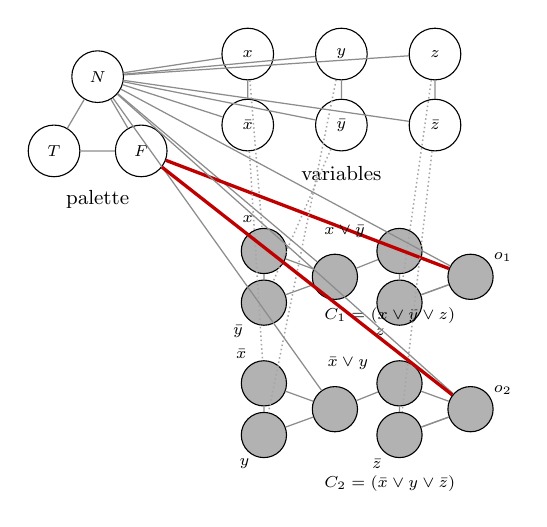
\begin{tikzpicture}[
  scale=0.82,
  transform shape,
  vertex/.style={circle, draw, minimum size=8mm, inner sep=0pt, font=\scriptsize},
  aux/.style={circle, draw, minimum size=7mm, inner sep=0pt, font=\scriptsize},
  ornode/.style={circle, draw, fill=black!30, minimum size=7mm, inner sep=0pt,
    font=\scriptsize},
  gate/.style={rectangle, draw, minimum width=13mm, minimum height=8mm,
    inner sep=1pt, font=\scriptsize},
  edge/.style={draw=black!45, line width=0.45pt},
  restrict/.style={draw=red!75!black, line width=1.2pt},
  feed/.style={draw=black!35, densely dotted, line width=0.55pt}
]
  % Palette.
  \node[vertex] (T) at (0,4.6) {$T$};
  \node[vertex] (F) at (1.35,4.6) {$F$};
  \node[vertex] (N) at (0.675,5.75) {$N$};
  \draw[edge] (T)--(F)--(N)--(T);
  \node[font=\small] at (0.675,3.85) {palette};

  % Variables.
  \node[vertex] (x) at (3.0,6.1) {$x$};
  \node[vertex] (nx) at (3.0,5.0) {$\bar x$};
  \node[vertex] (y) at (4.45,6.1) {$y$};
  \node[vertex] (ny) at (4.45,5.0) {$\bar y$};
  \node[vertex] (z) at (5.9,6.1) {$z$};
  \node[vertex] (nz) at (5.9,5.0) {$\bar z$};
  \foreach \a/\b in {x/nx,y/ny,z/nz}{
    \draw[edge] (\a)--(\b);
    \draw[edge] (\a)--(N);
    \draw[edge] (\b)--(N);
  }
  \node[font=\small] at (4.45,4.25) {variables};

  % Clause 1 complete OR-gadget chain.
  \node[ornode] (c1a) at (3.25,3.05) {};
  \node[ornode] (c1b) at (3.25,2.25) {};
  \node[ornode] (u1) at (4.35,2.65) {};
  \node[ornode] (c1u) at (5.35,3.05) {};
  \node[ornode] (c1c) at (5.35,2.25) {};
  \node[ornode] (o1) at (6.45,2.65) {};
  \draw[edge] (c1a)--(c1b)--(u1)--(c1a);
  \draw[edge] (u1)--(c1u)--(c1c)--(o1)--(c1u);
  \draw[edge] (c1c)--(o1);
  \draw[feed] (x)--(c1a);
  \draw[feed] (ny)--(c1b);
  \draw[feed] (z)--(c1c);
  \draw[edge] (u1)--(N);
  \draw[edge] (o1)--(N);
  \draw[restrict] (o1)--(F);
  \node[font=\scriptsize] at (3.0,3.55) {$x$};
  \node[font=\scriptsize] at (2.85,1.8) {$\bar y$};
  \node[font=\scriptsize] at (5.05,1.8) {$z$};
  \node[font=\scriptsize] at (4.5,3.35) {$x\vee \bar y$};
  \node[font=\scriptsize] at (6.95,2.95) {$o_1$};
  \node[font=\scriptsize] at (5.2,2.05) {$C_1=(x\vee \bar y\vee z)$};

  % Clause 2 complete OR-gadget chain.
  \node[ornode] (c2a) at (3.25,1.0) {};
  \node[ornode] (c2b) at (3.25,0.2) {};
  \node[ornode] (u2) at (4.35,0.6) {};
  \node[ornode] (c2u) at (5.35,1.0) {};
  \node[ornode] (c2c) at (5.35,0.2) {};
  \node[ornode] (o2) at (6.45,0.6) {};
  \draw[edge] (c2a)--(c2b)--(u2)--(c2a);
  \draw[edge] (u2)--(c2u)--(c2c)--(o2)--(c2u);
  \draw[edge] (c2c)--(o2);
  \draw[feed] (nx)--(c2a);
  \draw[feed] (y)--(c2b);
  \draw[feed] (nz)--(c2c);
  \draw[edge] (u2)--(N);
  \draw[edge] (o2)--(N);
  \draw[restrict] (o2)--(F);
  \node[font=\scriptsize] at (2.9,1.45) {$\bar x$};
  \node[font=\scriptsize] at (2.95,-0.25) {$y$};
  \node[font=\scriptsize] at (5.0,-0.25) {$\bar z$};
  \node[font=\scriptsize] at (4.55,1.3) {$\bar x\vee y$};
  \node[font=\scriptsize] at (6.95,0.9) {$o_2$};
  \node[font=\scriptsize] at (5.2,-0.55) {$C_2=(\bar x\vee y\vee \bar z)$};
\end{tikzpicture}
\end{center}

In the figure, each group of gray vertices is a complete OR-gadget. The first
triangle computes the OR of the first two literals, and the second triangle
combines that value with the third literal. The intermediate and final outputs
are connected to $N$, and the red edges connect the final clause outputs to
$F$.

The key point is the final red edge. If a clause has all three literals colored
False, then the OR-gadgets force its output $o_i$ to be colored False. But
$o_i$ is adjacent to the palette vertex $F$, so this is impossible in a proper
3-coloring. On the other hand, if at least one literal in the clause is True,
the OR-gadgets allow the output to be colored True, which is compatible with
the edges to $N$ and $F$.

Therefore, the graph is 3-colorable if and only if the original formula is
satisfiable. The construction uses a constant-size gadget for each variable
and each clause, so it is polynomial time. Since $3SAT$ is NP-complete, this
shows that $3COLOR$ is NP-hard. Together with $3COLOR\in NP$, we conclude that
$3COLOR$ is NP-complete.
\end{solution}

\end{document}
